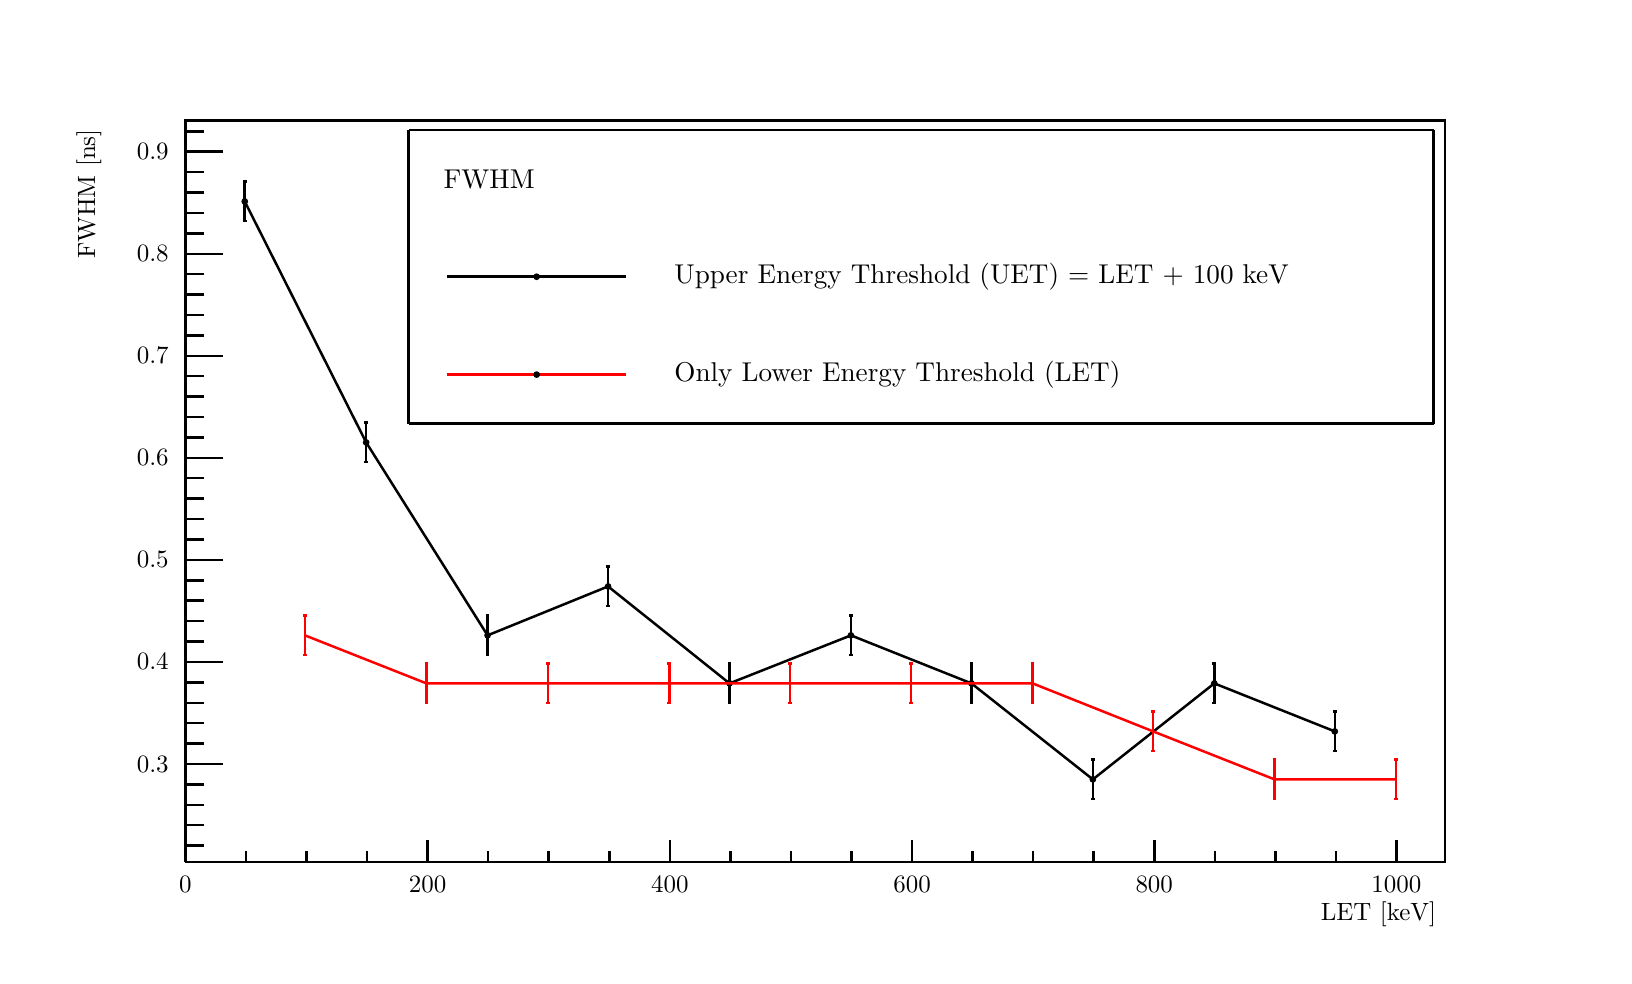
\begin{tikzpicture}
\pgfdeclareplotmark{cross} {
\pgfpathmoveto{\pgfpoint{-0.3\pgfplotmarksize}{\pgfplotmarksize}}
\pgfpathlineto{\pgfpoint{+0.3\pgfplotmarksize}{\pgfplotmarksize}}
\pgfpathlineto{\pgfpoint{+0.3\pgfplotmarksize}{0.3\pgfplotmarksize}}
\pgfpathlineto{\pgfpoint{+1\pgfplotmarksize}{0.3\pgfplotmarksize}}
\pgfpathlineto{\pgfpoint{+1\pgfplotmarksize}{-0.3\pgfplotmarksize}}
\pgfpathlineto{\pgfpoint{+0.3\pgfplotmarksize}{-0.3\pgfplotmarksize}}
\pgfpathlineto{\pgfpoint{+0.3\pgfplotmarksize}{-1.\pgfplotmarksize}}
\pgfpathlineto{\pgfpoint{-0.3\pgfplotmarksize}{-1.\pgfplotmarksize}}
\pgfpathlineto{\pgfpoint{-0.3\pgfplotmarksize}{-0.3\pgfplotmarksize}}
\pgfpathlineto{\pgfpoint{-1.\pgfplotmarksize}{-0.3\pgfplotmarksize}}
\pgfpathlineto{\pgfpoint{-1.\pgfplotmarksize}{0.3\pgfplotmarksize}}
\pgfpathlineto{\pgfpoint{-0.3\pgfplotmarksize}{0.3\pgfplotmarksize}}
\pgfpathclose
\pgfusepathqstroke
}
\pgfdeclareplotmark{cross*} {
\pgfpathmoveto{\pgfpoint{-0.3\pgfplotmarksize}{\pgfplotmarksize}}
\pgfpathlineto{\pgfpoint{+0.3\pgfplotmarksize}{\pgfplotmarksize}}
\pgfpathlineto{\pgfpoint{+0.3\pgfplotmarksize}{0.3\pgfplotmarksize}}
\pgfpathlineto{\pgfpoint{+1\pgfplotmarksize}{0.3\pgfplotmarksize}}
\pgfpathlineto{\pgfpoint{+1\pgfplotmarksize}{-0.3\pgfplotmarksize}}
\pgfpathlineto{\pgfpoint{+0.3\pgfplotmarksize}{-0.3\pgfplotmarksize}}
\pgfpathlineto{\pgfpoint{+0.3\pgfplotmarksize}{-1.\pgfplotmarksize}}
\pgfpathlineto{\pgfpoint{-0.3\pgfplotmarksize}{-1.\pgfplotmarksize}}
\pgfpathlineto{\pgfpoint{-0.3\pgfplotmarksize}{-0.3\pgfplotmarksize}}
\pgfpathlineto{\pgfpoint{-1.\pgfplotmarksize}{-0.3\pgfplotmarksize}}
\pgfpathlineto{\pgfpoint{-1.\pgfplotmarksize}{0.3\pgfplotmarksize}}
\pgfpathlineto{\pgfpoint{-0.3\pgfplotmarksize}{0.3\pgfplotmarksize}}
\pgfpathclose
\pgfusepathqfillstroke
}
\pgfdeclareplotmark{newstar} {
\pgfpathmoveto{\pgfqpoint{0pt}{\pgfplotmarksize}}
\pgfpathlineto{\pgfqpointpolar{44}{0.5\pgfplotmarksize}}
\pgfpathlineto{\pgfqpointpolar{18}{\pgfplotmarksize}}
\pgfpathlineto{\pgfqpointpolar{-20}{0.5\pgfplotmarksize}}
\pgfpathlineto{\pgfqpointpolar{-54}{\pgfplotmarksize}}
\pgfpathlineto{\pgfqpointpolar{-90}{0.5\pgfplotmarksize}}
\pgfpathlineto{\pgfqpointpolar{234}{\pgfplotmarksize}}
\pgfpathlineto{\pgfqpointpolar{198}{0.5\pgfplotmarksize}}
\pgfpathlineto{\pgfqpointpolar{162}{\pgfplotmarksize}}
\pgfpathlineto{\pgfqpointpolar{134}{0.5\pgfplotmarksize}}
\pgfpathclose
\pgfusepathqstroke
}
\pgfdeclareplotmark{newstar*} {
\pgfpathmoveto{\pgfqpoint{0pt}{\pgfplotmarksize}}
\pgfpathlineto{\pgfqpointpolar{44}{0.5\pgfplotmarksize}}
\pgfpathlineto{\pgfqpointpolar{18}{\pgfplotmarksize}}
\pgfpathlineto{\pgfqpointpolar{-20}{0.5\pgfplotmarksize}}
\pgfpathlineto{\pgfqpointpolar{-54}{\pgfplotmarksize}}
\pgfpathlineto{\pgfqpointpolar{-90}{0.5\pgfplotmarksize}}
\pgfpathlineto{\pgfqpointpolar{234}{\pgfplotmarksize}}
\pgfpathlineto{\pgfqpointpolar{198}{0.5\pgfplotmarksize}}
\pgfpathlineto{\pgfqpointpolar{162}{\pgfplotmarksize}}
\pgfpathlineto{\pgfqpointpolar{134}{0.5\pgfplotmarksize}}
\pgfpathclose
\pgfusepathqfillstroke
}
\definecolor{c}{rgb}{1,1,1};
\draw [color=c, fill=c] (0,0) rectangle (20,11.7753);
\draw [color=c, fill=c] (1.99641,1.1835) rectangle (17.9916,10.6037);
\definecolor{c}{rgb}{0,0,0};
\draw [c,line width=0.9] (1.99641,1.1835) -- (1.99641,10.6037) -- (17.9916,10.6037) -- (17.9916,1.1835) -- (1.99641,1.1835);
\definecolor{c}{rgb}{1,1,1};
\draw [color=c, fill=c] (1.99641,1.1835) rectangle (17.9916,10.6037);
\definecolor{c}{rgb}{0,0,0};
\draw [c,line width=0.9] (1.99641,1.1835) -- (1.99641,10.6037) -- (17.9916,10.6037) -- (17.9916,1.1835) -- (1.99641,1.1835);
\draw [c,line width=0.9] (1.99641,1.1835) -- (17.9916,1.1835);
\draw [c,line width=0.9] (1.99641,1.46602) -- (1.99641,1.1835);
\draw [c,line width=0.9] (2.76541,1.32476) -- (2.76541,1.1835);
\draw [c,line width=0.9] (3.53442,1.32476) -- (3.53442,1.1835);
\draw [c,line width=0.9] (4.30342,1.32476) -- (4.30342,1.1835);
\draw [c,line width=0.9] (5.07242,1.46602) -- (5.07242,1.1835);
\draw [c,line width=0.9] (5.84142,1.32476) -- (5.84142,1.1835);
\draw [c,line width=0.9] (6.61042,1.32476) -- (6.61042,1.1835);
\draw [c,line width=0.9] (7.37942,1.32476) -- (7.37942,1.1835);
\draw [c,line width=0.9] (8.14842,1.46602) -- (8.14842,1.1835);
\draw [c,line width=0.9] (8.91742,1.32476) -- (8.91742,1.1835);
\draw [c,line width=0.9] (9.68642,1.32476) -- (9.68642,1.1835);
\draw [c,line width=0.9] (10.4554,1.32476) -- (10.4554,1.1835);
\draw [c,line width=0.9] (11.2244,1.46602) -- (11.2244,1.1835);
\draw [c,line width=0.9] (11.9934,1.32476) -- (11.9934,1.1835);
\draw [c,line width=0.9] (12.7624,1.32476) -- (12.7624,1.1835);
\draw [c,line width=0.9] (13.5314,1.32476) -- (13.5314,1.1835);
\draw [c,line width=0.9] (14.3004,1.46602) -- (14.3004,1.1835);
\draw [c,line width=0.9] (15.0694,1.32476) -- (15.0694,1.1835);
\draw [c,line width=0.9] (15.8384,1.32476) -- (15.8384,1.1835);
\draw [c,line width=0.9] (16.6074,1.32476) -- (16.6074,1.1835);
\draw [c,line width=0.9] (17.3764,1.46602) -- (17.3764,1.1835);
\draw [c,line width=0.9] (17.3764,1.46602) -- (17.3764,1.1835);
\draw [anchor=base] (1.99641,0.794919) node[scale=0.902725, color=c, rotate=0]{0};
\draw [anchor=base] (5.07242,0.794919) node[scale=0.902725, color=c, rotate=0]{200};
\draw [anchor=base] (8.14842,0.794919) node[scale=0.902725, color=c, rotate=0]{400};
\draw [anchor=base] (11.2244,0.794919) node[scale=0.902725, color=c, rotate=0]{600};
\draw [anchor=base] (14.3004,0.794919) node[scale=0.902725, color=c, rotate=0]{800};
\draw [anchor=base] (17.3764,0.794919) node[scale=0.902725, color=c, rotate=0]{1000};
\draw [anchor= east] (17.9916,0.524089) node[scale=0.902725, color=c, rotate=0]{LET [keV]};
\draw [c,line width=0.9] (1.99641,1.1835) -- (1.99641,10.6037);
\draw [c,line width=0.9] (2.47641,2.43127) -- (1.99641,2.43127);
\draw [c,line width=0.9] (2.23641,2.69045) -- (1.99641,2.69045);
\draw [c,line width=0.9] (2.23641,2.94964) -- (1.99641,2.94964);
\draw [c,line width=0.9] (2.23641,3.20883) -- (1.99641,3.20883);
\draw [c,line width=0.9] (2.23641,3.46802) -- (1.99641,3.46802);
\draw [c,line width=0.9] (2.47641,3.72721) -- (1.99641,3.72721);
\draw [c,line width=0.9] (2.23641,3.98639) -- (1.99641,3.98639);
\draw [c,line width=0.9] (2.23641,4.24558) -- (1.99641,4.24558);
\draw [c,line width=0.9] (2.23641,4.50477) -- (1.99641,4.50477);
\draw [c,line width=0.9] (2.23641,4.76396) -- (1.99641,4.76396);
\draw [c,line width=0.9] (2.47641,5.02315) -- (1.99641,5.02315);
\draw [c,line width=0.9] (2.23641,5.28234) -- (1.99641,5.28234);
\draw [c,line width=0.9] (2.23641,5.54152) -- (1.99641,5.54152);
\draw [c,line width=0.9] (2.23641,5.80071) -- (1.99641,5.80071);
\draw [c,line width=0.9] (2.23641,6.0599) -- (1.99641,6.0599);
\draw [c,line width=0.9] (2.47641,6.31909) -- (1.99641,6.31909);
\draw [c,line width=0.9] (2.23641,6.57828) -- (1.99641,6.57828);
\draw [c,line width=0.9] (2.23641,6.83746) -- (1.99641,6.83746);
\draw [c,line width=0.9] (2.23641,7.09665) -- (1.99641,7.09665);
\draw [c,line width=0.9] (2.23641,7.35584) -- (1.99641,7.35584);
\draw [c,line width=0.9] (2.47641,7.61503) -- (1.99641,7.61503);
\draw [c,line width=0.9] (2.23641,7.87422) -- (1.99641,7.87422);
\draw [c,line width=0.9] (2.23641,8.1334) -- (1.99641,8.1334);
\draw [c,line width=0.9] (2.23641,8.39259) -- (1.99641,8.39259);
\draw [c,line width=0.9] (2.23641,8.65178) -- (1.99641,8.65178);
\draw [c,line width=0.9] (2.47641,8.91097) -- (1.99641,8.91097);
\draw [c,line width=0.9] (2.23641,9.17016) -- (1.99641,9.17016);
\draw [c,line width=0.9] (2.23641,9.42934) -- (1.99641,9.42934);
\draw [c,line width=0.9] (2.23641,9.68853) -- (1.99641,9.68853);
\draw [c,line width=0.9] (2.23641,9.94772) -- (1.99641,9.94772);
\draw [c,line width=0.9] (2.47641,10.2069) -- (1.99641,10.2069);
\draw [c,line width=0.9] (2.47641,2.43127) -- (1.99641,2.43127);
\draw [c,line width=0.9] (2.23641,2.17208) -- (1.99641,2.17208);
\draw [c,line width=0.9] (2.23641,1.91289) -- (1.99641,1.91289);
\draw [c,line width=0.9] (2.23641,1.6537) -- (1.99641,1.6537);
\draw [c,line width=0.9] (2.23641,1.39451) -- (1.99641,1.39451);
\draw [c,line width=0.9] (2.47641,10.2069) -- (1.99641,10.2069);
\draw [c,line width=0.9] (2.23641,10.4661) -- (1.99641,10.4661);
\draw [anchor= east] (1.89641,2.43127) node[scale=0.902725, color=c, rotate=0]{0.3};
\draw [anchor= east] (1.89641,3.72721) node[scale=0.902725, color=c, rotate=0]{0.4};
\draw [anchor= east] (1.89641,5.02315) node[scale=0.902725, color=c, rotate=0]{0.5};
\draw [anchor= east] (1.89641,6.31909) node[scale=0.902725, color=c, rotate=0]{0.6};
\draw [anchor= east] (1.89641,7.61503) node[scale=0.902725, color=c, rotate=0]{0.7};
\draw [anchor= east] (1.89641,8.91097) node[scale=0.902725, color=c, rotate=0]{0.8};
\draw [anchor= east] (1.89641,10.2069) node[scale=0.902725, color=c, rotate=0]{0.9};
\draw [anchor= east] (0.770412,10.6037) node[scale=0.902725, color=c, rotate=90]{FWHM [ns]};
\draw [c,line width=0.9] (2.74955,9.57561) -- (4.29169,6.51524) -- (5.83383,4.06455) -- (7.36402,4.68619) -- (8.90616,3.45487) -- (10.4483,4.06455) -- (11.9785,3.45487) -- (13.5206,2.23551) -- (15.0628,3.45487) -- (16.5929,2.84519);
\foreach \P in {(2.74955,9.57561), (4.29169,6.51524), (5.83383,4.06455), (7.36402,4.68619), (8.90616,3.45487), (10.4483,4.06455), (11.9785,3.45487), (13.5206,2.23551), (15.0628,3.45487), (16.5929,2.84519)}{\draw[mark options={color=c,fill=c},mark
 size=2.402402pt,mark=*,mark size=1pt] plot coordinates {\P};}
\draw [c,line width=0.9] (2.74955,9.57561) -- (2.74955,9.82562);
\draw [c,line width=0.9] (2.72564,9.82562) -- (2.77346,9.82562);
\draw [c,line width=0.9] (2.74955,9.57561) -- (2.74955,9.32561);
\draw [c,line width=0.9] (2.72564,9.32561) -- (2.77346,9.32561);
\draw [c,line width=0.9] (4.29169,6.51524) -- (4.29169,6.76525);
\draw [c,line width=0.9] (4.26778,6.76525) -- (4.3156,6.76525);
\draw [c,line width=0.9] (4.29169,6.51524) -- (4.29169,6.26524);
\draw [c,line width=0.9] (4.26778,6.26524) -- (4.3156,6.26524);
\draw [c,line width=0.9] (5.83383,4.06455) -- (5.83383,4.31456);
\draw [c,line width=0.9] (5.80992,4.31456) -- (5.85774,4.31456);
\draw [c,line width=0.9] (5.83383,4.06455) -- (5.83383,3.81455);
\draw [c,line width=0.9] (5.80992,3.81455) -- (5.85774,3.81455);
\draw [c,line width=0.9] (7.36402,4.68619) -- (7.36402,4.9362);
\draw [c,line width=0.9] (7.34011,4.9362) -- (7.38793,4.9362);
\draw [c,line width=0.9] (7.36402,4.68619) -- (7.36402,4.43619);
\draw [c,line width=0.9] (7.34011,4.43619) -- (7.38793,4.43619);
\draw [c,line width=0.9] (8.90616,3.45487) -- (8.90616,3.70488);
\draw [c,line width=0.9] (8.88225,3.70488) -- (8.93007,3.70488);
\draw [c,line width=0.9] (8.90616,3.45487) -- (8.90616,3.20487);
\draw [c,line width=0.9] (8.88225,3.20487) -- (8.93007,3.20487);
\draw [c,line width=0.9] (10.4483,4.06455) -- (10.4483,4.31456);
\draw [c,line width=0.9] (10.4244,4.31456) -- (10.4722,4.31456);
\draw [c,line width=0.9] (10.4483,4.06455) -- (10.4483,3.81455);
\draw [c,line width=0.9] (10.4244,3.81455) -- (10.4722,3.81455);
\draw [c,line width=0.9] (11.9785,3.45487) -- (11.9785,3.70488);
\draw [c,line width=0.9] (11.9546,3.70488) -- (12.0024,3.70488);
\draw [c,line width=0.9] (11.9785,3.45487) -- (11.9785,3.20487);
\draw [c,line width=0.9] (11.9546,3.20487) -- (12.0024,3.20487);
\draw [c,line width=0.9] (13.5206,2.23551) -- (13.5206,2.48551);
\draw [c,line width=0.9] (13.4967,2.48551) -- (13.5445,2.48551);
\draw [c,line width=0.9] (13.5206,2.23551) -- (13.5206,1.9855);
\draw [c,line width=0.9] (13.4967,1.9855) -- (13.5445,1.9855);
\draw [c,line width=0.9] (15.0628,3.45487) -- (15.0628,3.70488);
\draw [c,line width=0.9] (15.0389,3.70488) -- (15.0867,3.70488);
\draw [c,line width=0.9] (15.0628,3.45487) -- (15.0628,3.20487);
\draw [c,line width=0.9] (15.0389,3.20487) -- (15.0867,3.20487);
\draw [c,line width=0.9] (16.5929,2.84519) -- (16.5929,3.09519);
\draw [c,line width=0.9] (16.569,3.09519) -- (16.6169,3.09519);
\draw [c,line width=0.9] (16.5929,2.84519) -- (16.5929,2.59518);
\draw [c,line width=0.9] (16.569,2.59518) -- (16.6169,2.59518);
\definecolor{c}{rgb}{1,0,0};
\draw [c,line width=0.9] (3.51464,4.06455) -- (3.51464,4.31456);
\draw [c,line width=0.9] (3.49074,4.31456) -- (3.53855,4.31456);
\draw [c,line width=0.9] (3.51464,4.06455) -- (3.51464,3.81455);
\draw [c,line width=0.9] (3.49074,3.81455) -- (3.53855,3.81455);
\draw [c,line width=0.9] (5.05678,3.45487) -- (5.05678,3.70488);
\draw [c,line width=0.9] (5.03288,3.70488) -- (5.08069,3.70488);
\draw [c,line width=0.9] (5.05678,3.45487) -- (5.05678,3.20487);
\draw [c,line width=0.9] (5.03288,3.20487) -- (5.08069,3.20487);
\draw [c,line width=0.9] (6.59892,3.45487) -- (6.59892,3.70488);
\draw [c,line width=0.9] (6.57502,3.70488) -- (6.62283,3.70488);
\draw [c,line width=0.9] (6.59892,3.45487) -- (6.59892,3.20487);
\draw [c,line width=0.9] (6.57502,3.20487) -- (6.62283,3.20487);
\draw [c,line width=0.9] (8.14106,3.45487) -- (8.14106,3.70488);
\draw [c,line width=0.9] (8.11716,3.70488) -- (8.16497,3.70488);
\draw [c,line width=0.9] (8.14106,3.45487) -- (8.14106,3.20487);
\draw [c,line width=0.9] (8.11716,3.20487) -- (8.16497,3.20487);
\draw [c,line width=0.9] (9.67125,3.45487) -- (9.67125,3.70488);
\draw [c,line width=0.9] (9.64734,3.70488) -- (9.69516,3.70488);
\draw [c,line width=0.9] (9.67125,3.45487) -- (9.67125,3.20487);
\draw [c,line width=0.9] (9.64734,3.20487) -- (9.69516,3.20487);
\draw [c,line width=0.9] (11.2134,3.45487) -- (11.2134,3.70488);
\draw [c,line width=0.9] (11.1895,3.70488) -- (11.2373,3.70488);
\draw [c,line width=0.9] (11.2134,3.45487) -- (11.2134,3.20487);
\draw [c,line width=0.9] (11.1895,3.20487) -- (11.2373,3.20487);
\draw [c,line width=0.9] (12.7555,3.45487) -- (12.7555,3.70488);
\draw [c,line width=0.9] (12.7316,3.70488) -- (12.7794,3.70488);
\draw [c,line width=0.9] (12.7555,3.45487) -- (12.7555,3.20487);
\draw [c,line width=0.9] (12.7316,3.20487) -- (12.7794,3.20487);
\draw [c,line width=0.9] (14.2857,2.84519) -- (14.2857,3.09519);
\draw [c,line width=0.9] (14.2618,3.09519) -- (14.3096,3.09519);
\draw [c,line width=0.9] (14.2857,2.84519) -- (14.2857,2.59518);
\draw [c,line width=0.9] (14.2618,2.59518) -- (14.3096,2.59518);
\draw [c,line width=0.9] (15.8279,2.23551) -- (15.8279,2.48551);
\draw [c,line width=0.9] (15.8039,2.48551) -- (15.8518,2.48551);
\draw [c,line width=0.9] (15.8279,2.23551) -- (15.8279,1.9855);
\draw [c,line width=0.9] (15.8039,1.9855) -- (15.8518,1.9855);
\draw [c,line width=0.9] (17.37,2.23551) -- (17.37,2.48551);
\draw [c,line width=0.9] (17.3461,2.48551) -- (17.3939,2.48551);
\draw [c,line width=0.9] (17.37,2.23551) -- (17.37,1.9855);
\draw [c,line width=0.9] (17.3461,1.9855) -- (17.3939,1.9855);
\draw [c,line width=0.9] (3.51464,4.06455) -- (5.05678,3.45487) -- (6.59892,3.45487) -- (8.14106,3.45487) -- (9.67125,3.45487) -- (11.2134,3.45487) -- (12.7555,3.45487) -- (14.2857,2.84519) -- (15.8279,2.23551) -- (17.37,2.23551);
\definecolor{c}{rgb}{1,1,1};
\draw [color=c, fill=c] (4.82965,6.75433) rectangle (17.8482,10.4842);
\definecolor{c}{rgb}{0,0,0};
\draw [c,line width=0.9] (4.82965,6.75433) -- (17.8482,6.75433);
\draw [c,line width=0.9] (17.8482,6.75433) -- (17.8482,10.4842);
\draw [c,line width=0.9] (17.8482,10.4842) -- (4.82965,10.4842);
\draw [c,line width=0.9] (4.82965,10.4842) -- (4.82965,6.75433);
\draw [anchor= west] (5.15511,9.86252) node[scale=0.982378, color=c, rotate=0]{FWHM};
\draw [anchor= west] (8.08428,8.61925) node[scale=0.982378, color=c, rotate=0]{Upper Energy Threshold (UET) = LET + 100 keV};
\definecolor{c}{rgb}{1,1,1};
\draw [c, fill=c] (5.31784,8.1841) -- (7.59609,8.1841) -- (7.59609,9.05439) -- (5.31784,9.05439);
\definecolor{c}{rgb}{0,0,0};
\draw [c,line width=0.9] (5.31784,8.61925) -- (7.59609,8.61925);
\foreach \P in {(6.45696,8.61925)}{\draw[mark options={color=c,fill=c},mark size=2.402402pt,mark=*,mark size=1pt] plot coordinates {\P};}
\draw [anchor= west] (8.08428,7.37597) node[scale=0.982378, color=c, rotate=0]{Only Lower Energy Threshold (LET)};
\definecolor{c}{rgb}{1,1,1};
\draw [c, fill=c] (5.31784,6.94082) -- (7.59609,6.94082) -- (7.59609,7.81112) -- (5.31784,7.81112);
\definecolor{c}{rgb}{1,0,0};
\draw [c,line width=0.9] (5.31784,7.37597) -- (7.59609,7.37597);
\definecolor{c}{rgb}{0,0,0};
\foreach \P in {(6.45696,7.37597)}{\draw[mark options={color=c,fill=c},mark size=2.402402pt,mark=*,mark size=1pt] plot coordinates {\P};}
\end{tikzpicture}
